
\documentclass{article}
\usepackage{graphicx}
\graphicspath{ {figures/} }
\usepackage{enumitem}
\usepackage{hyperref}
\usepackage{comment}
\usepackage{xcolor}
\usepackage[utf8]{inputenc}
\usepackage[paper size={180mm, 240mm},left=25mm,right=25mm,top=35mm,bottom=25mm,nohea d]{geometry}
\usepackage{tabularx}
\usepackage{algpseudocode}
\usepackage{algorithm}
\usepackage{amsmath}
\usepackage{amssymb}
\usepackage{pdflscape}

\newenvironment{myfontAPI}{\fontfamily{LinuxBiolinumT-OsF}\selectfont}{\par}

%\renewcommand{\familydefault}{\sfdefault}%

\makeatletter
\def\namedlabel#1#2{\begingroup
    #2%
    \def\@currentlabel{#2}%
    \phantomsection\label{#1}\endgroup
}
\makeatother

\title{ Code Inspection Document  
\\ ``MyTaxiService'' Application
\\ A.Y. 2015 - 2016 }

\author{Ennio Visconti (mat. 790382)
\\ Simone Zocchi (mat. 852910)
\\ Khanh Huy Paolo Tran (mat. 852496)}

\date{\today}
\makeatletter
\def\namedlabel#1#2{\begingroup
    #2%
    \def\@currentlabel{#2}%
    \phantomsection\label{#1}\endgroup
}
\makeatother

\bibliographystyle{plain}

\begin{document}
   
    \begin{titlepage}
        \maketitle 
        \vfill
        \centerline{
\includegraphics[scale=0.5]{LogoPolimi}}
        \vfill
        \vfill
    \end{titlepage}

        
    \tableofcontents

% --------------------------------------------------
% PLEASE REMEMBER TO UPDATE TIME SPENT IN time.tex
% --------------------------------------------------

\section{Introduction}

\subsection{Purpose}
This document has the \textbf{goal} of providing an overall and complete description of \textit{myTaxiService}'s software architectural design together with algorithms and UI.\\
The intended audience of this document are project managers and software developers.

\subsection{Scope}
\textit{myTaxiService} is an application born to support an existing taxi company, especially to simplify passengers' access to the service and guarantee a fair management of taxi queues. In fact it will be GPS-based and it will be able to assign a taxi to a certain call, based on the location of the taxi and of the requesting passenger, in order to minimize the waiting time.\\
It will also provide an option to reserve a taxi in advance and to share the ride with other passengers to save money. All these features will be available via a freely downloadable mobile application or a web application.\\
It will also provide an interface for the taxi drivers, in order to communicate with them more easily and to make them able to automatically share their location over time.

\subsection{Definitions, Acronyms, Abbreviations}

\subsubsection{Definitions}
\begin{itemize}
\item \textbf{Dynamic queue}: it is a list of taxis which is created whenever a request must be managed.
\item \textbf{Static queue}: it is a list of taxis which is associated to every zones. 
\end{itemize}

\subsubsection{Acronyms \& Abbreviations}
\begin{itemize}
\item \textbf{UML}: Unified Modeling Language
\item \textbf{API}: Application Programming Interface
\item \textbf{MVC}: Model - View - Controller
\item \textbf{DTO}: Data Transfer Object
\item \textbf{PSP}: Payment Service Provider
\end{itemize}


\subsection{Document Structure}
The document divides into 5 parts:
\begin{itemize}

\item Section 1: \textbf{Introduction}. It gives a description of the document underlining his goals and gives basic information about the application.

\item Section 2: \textbf{Architectural Design}. It gives the various architectural views of the application.

\item Section 3: \textbf{Algorithm Design}. It gives some algorithms' descriptions contained in the application.

\item Section 4: \textbf{User Interface Design}. It shows application's mockups.

\item Section 5: \textbf{Requirements Traceability}. It contains solutions to the RASD requirements.

\item Section 6: \textbf{References}. It contains all DD's references.

\end{itemize}



\section{Functional Description}
The following information were taken from the JavaDoc of the interface EntityResolver in the package org.xml.sax, from "Oracle GlassFish Server 3.1 "Application Deployment Guide" and from a step by step reading of the code.
\subsection{Context Overview}
This procedure is used during the deployment of a web application. It extracts the configurations of application-scoped resources from an xml document named \textit{glassfish-resources.xml}, which has the following structure (only relevant elements has been considered):\\\\
\begin{myfontAPI}
resources \\
{[}. . .{]}\\
.\indent resource-adapter-config\\
.\indent .\indent property (with attributes)\\
.\indent .\indent .\indent Description\\
.\indent connector-connection-pool\\
.\indent .\indent Description\\
.\indent .\indent security-map\\
.\indent .\indent .\indent Principal\\
.\indent .\indent .\indent user-group\\
.\indent .\indent .\indent backend-principal\\
.\indent .\indent property (with attributes)\\
.\indent .\indent .\indent Description\\
.\indent work-security-map\\
.\indent .\indent Description\\
.\indent .\indent principal-map\\
.\indent .\indent group-map\\
\end{myfontAPI}

Application-scoped resources are all the modules and other applications which are required at deployment time, they are created during the deployment phase and destroyed at its completion, they are available only to the module or application which defines it.

\subsection{Class Overview}
The class we have inspected is an implementation of the interface \textit{EntityResolver} provided by the SAX java package.\\
It should be used by an XML parser to intercept any external entities before including them. The \textit{resolveEntity} method is the implementation of this aspect.\\

When the constructor of this class is invoked with a source file as a parameter, which must be an XML document, the file is parsed and all the nodes are copied into a collection of objects called \textit{vResource}, with all the attributes that the nodes have, and in a Map with all the their child nodes' references. The three generate* methods are an implementation of what just said, for three specific type of nodes. For further information see Figure~\ref{fig:flowchart}.

\begin{figure}[]
        \centering
        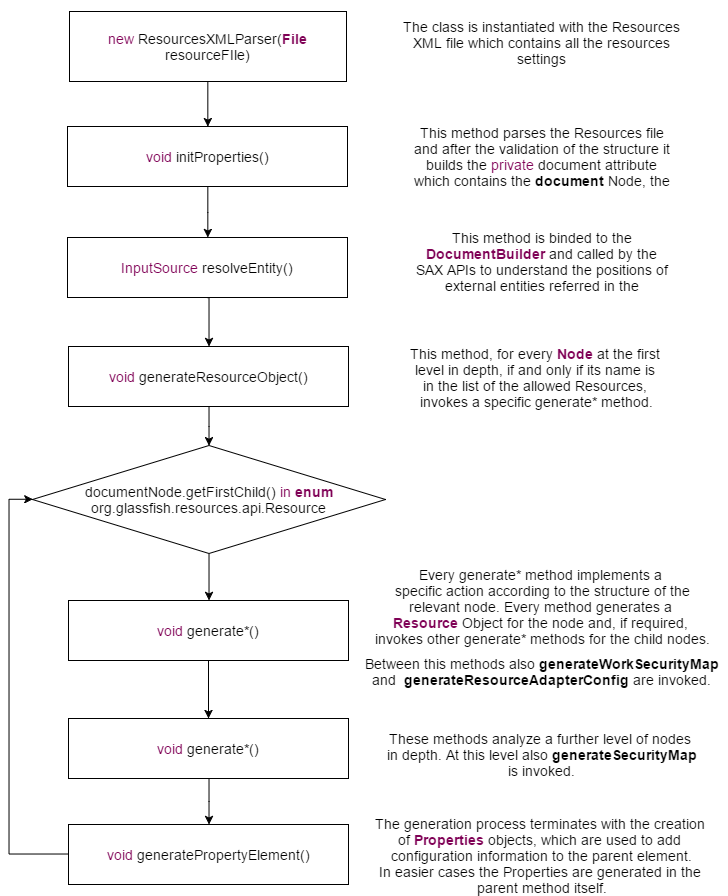
\includegraphics[width=1\columnwidth]{FlowChart}
        \caption{High level flow chart of class execution}
        \label{fig:flowchart}
\end{figure}

\subsection{Method: resolveEntity}
In the resolveEntity method, firstly, the DTD version is identified, comparing the publicId and systemId parameters with a preset list of names, and then if the DTD file is present, it is loaded as an InputStream otherwise an Exception is thrown.

\subsection{Method: generateWorkSecurityMap}
The method generateWorkSecurityMap is called by generateResourceObjects if the name of the node in exam is CONNECTOR\_WORK\_SECURITY\_MAP. It creates a Resource object and sets two attributes of the object with the value of the relevant attributes of the node. Then for all the children nodes that are \\WORK\_SECURITY\_MAP\_GROUP\_MAP or \\WORK\_SECURITY\_MAP\_PRINCIPAL\_MAP it add other attributes to the resource with the value of the relevant nodes.\\
Finally the resource is added to the collection of resources and to the map.

\subsection{Method: generateSecurityMap}
The method generateSecurityMap is called by generateConnectorConnectionPoolResource if the name of the node in exam is SECURITY\_MAP. A resource for the node is created and few basic attributes of the resource are added. Then the children nodes are extracted and if their names are SECURITY\_MAP\_PRINCIPAL or SECURITY\_MAP\_USER\_GROUP the first child is extracted and the value inserted in a String array that are then inserted as attributes of the Resource. If the child node is, instead, a SECURITY\_MAP\_BACKEND\_PRINCIPAL, the values of its attributes USER\_NAME and PASSWORD are directly added as attributes of the resource. The resource is finally added to the collection of resources and to the map.

\subsection{Method: generateResourceAdapterConfig}
The method generateResourceAdapterConfig is called by generateResourceObjects if the name of the node in exam is RESOURCE\_ADAPTER\_CONFIG. As before, a Resource element is created and the attributes of the nodes are added to the resource. The resource is then added to the the collection of resources and to the map.

\section{Issues Analysis}

\subsection{Issue Categories}

\subsubsection{Naming Conventions}
    \begin{itemize}

\item [1-7.] Naming convention has been correctly taken into account. In fact constants are always in upper case and the classic camel case standard is used (upper camel case for class and interface names and lower camel case for variable names and parameters) with the only exception of a variable at \textit{line 1403}. Furthermore all the constants, variables, classes and interfaces used or defined have a name that clearly explains their meaning.

\end{itemize}

% Analisi di dettaglio %
\begin{comment}

\begin{itemize}
\item [1.] Names are all meaningful in the context of the code and the given JavaDoc.
\item [2.] All one-character variables are used for temporary "throwaway" variables.
\item [3. - 4.] Classical camel-upper-case standard is followed for both classes and interfaces.
\item [5.] Methods are verbs with the first letter of each addition word capitalize.
\item [6.] Variables have following word in lower case. 
\item [7.] Constants are all in upper case.
\end{itemize}

\end{comment}
    
\subsubsection{Indentation}
    \begin{itemize}
\item [8.] Indentations are done with 4 spaces.
\item [9.] No tabs are used (besides \textit{line 234}, which isn't in our assignment).
\end{itemize}
    
\subsubsection{Braces}
    \begin{itemize}
\item [10-11.] “Kernighan and Ritchie” style is used but is not really consistent, like on method definitions at \textit{lines 1448, 1533}. Furthermore in a few cases control blocks have no curly braces because they are executing a single statements, like at \textit{lines 1389, 1400, 1453}.
\end{itemize}
    
    
\subsubsection{File Organization}
    \begin{itemize}
\item [12.] Use of blank lines and comments is not very frequent in the class analyzed. When used, they properly separate sections in the class.
\item [13.] Practical lines in a few cases exceed the maximum length of 80 characters, for example at \textit{lines 1328, 1336, 1349, 1363, 1364, 1372, 1383, 1394, 1455, 1626}
\item [14.] In a few cases, for instance in method declaration, they also exceed the 120 char maximum length. \textit{Lines 964, 1191, 1524}  

\end{itemize}
    
\subsubsection{Wrapping Lines}
    \begin{itemize}
\item [15.] Line breaks are always used in the correct way, after '+' \textit{at lines 1598-1600}, or ',' \textit{ at lines 1227, 1232, 1506, 1524...}
\item [16.] When too long, parenthesized expressions are wrapped accordingly to the parenthesis hierarchy.
\item [17.] Not always new statements are aligned with the beginning of the expression at the same level as the previous lines, like at \textit{lines 1260, 1436, 1437, 1439}.
\end{itemize}
    
\subsubsection{Comments}
    \begin{itemize}
\item [18.] There are no comments explaining what the code is doing. \textit{Lines 1319, 1385, 1449}.

\item [19.] Outside our code block there is commented out code. It doesn't contain neither reasons for being eliminated nor date for the definitive elimination. \textit{Lines 243, 1107}. 

\end{itemize}
    
\subsubsection{Java Source Files}
    \begin{itemize}
\item [20-21.] The only file of our block contains just three classes and no interfaces of which the only public class is the first.
\item [22.] The method resolveEntity is consistent with the javadoc, besides it doesn't throw \textit{IOException}.
\item [23.] The javadoc doesn't cover \textit{generateWorkSecurityMap}, \textit{generateSecurityMap} and \textit{generateResourceAdapterConfig} probably because they are private methods.
\end{itemize}
    
\subsubsection{Package and Import Statements}
    \begin{itemize}
\item [24.] In the given class the package statement is correctly placed at the beginning of the document, only after the introductory comment. It is correctly followed by all the import statements.
\end{itemize}
    
\subsubsection{Class and Interface Declarations}
    \begin{itemize}
\item [25.]  A first comment with the explanation of the class is present, followed by the package location and the import statements. The documentation comment is present but is very short and not complete.\\
As the class is an implementation of EntityResolver interface, the implementation comment should be provided but it is not present.\\
Class (static) variables and instance variables are grouped but placed in the wrong order, firstly are placed the instance variables and then the class ones.\\
After that, methods are placed but, at the end of the document, they are mixed with the declarations of two inner classes.
\item [26.] The methods are not properly grouped by accessibility, for instance the most of the public methods are placed at the beginning of the class and a few of them are at the end.
They seems to be grouped by functionality, in fact there is a set of methods for generate resources, followed by some getter methods.
\item [27.] Methods \textit{generateWorkSecurityMap}, \textit{generateSecurityMap} and \textit{resolveEntity} are a little bit too long.\\
Encapsulation is preserved.\\
\textit{generateWorkSecurityMap} has an \textit{else if} which does basically the same thing as the precondition, but with a different node, so there are duplicated code lines. \textit{Lines 1344-1374}\\
In addition inside \textit{resolveEntity} there is a checking command repeated many times ( \textit{if(\_logger.isLoggable(Level.FINEST))} ). \textit{Lines 1601, 1606, 1611, 1619, 1625}.
\end{itemize}

    
\subsubsection{Initialization and Declarations}
    \begin{itemize}
\item [28.] All class members (of our code block) have the correct visibility (they are all private except the one defined in the interface implemented). All variables and class members are of the type required by their usage and so they can be considered as correct.
\item [29.] Variable scoping is done really well. Every variable is declared exactly when it is needed and never before.
\item [30.] Every new object is instantiated through the constructor.
\item [31-32.] All the variables are initialized immediately after the declaration. Furthermore the methods are always invoked with correct parameters and therefore parameters references are correctly initialized.
\item [33.] Some variables aren't declared at the beginning of a block. \textit{Lines 1339, 1405, 1472, 1609, 1616-1617, 1622}
\end{itemize}
    
\subsubsection{Method Calls}
    \begin{itemize}
\item [34.] All parameters are presented in the correct order.
\item [35.] All the correct methods are called.
\item [36.] Methods invoked in \textit{generateWorkSecurityMap}, \textit{generateSecurityMap} and \textit{generateResourceAdapterConfig}, whose returned value is then used, are only methods that extract Nodes, List of nodes or the value of a node as String. The values are then copied in local resources and maps, matching node types with their value.\\ In \textit{resolveEntity} are used methods to get items from a list, compare strings and create InputStream from URL. \\ The values are always used in a proper way.
\end{itemize}
    
\subsubsection{Arrays}
    \begin{itemize}
\item [37.] The collections used are always entirely scanned and the items of the collections are always accessed through the \textit{get(i)} or \textit{item(i)} methods. \textit{Lines 1342, 1409, 1420, 1579}.
\item [38.] The collections used are always scanned in for statements that use the exit condition \textit{i $<$ array.getLength()} (or \textit{array.size()}) with i=0 and incremented by one at every iteration. So no index goes out of bound. \textit{1341, 1408, 1578}.
\item [39.] No array is created and no elements are added to Collections used.
\end{itemize}
    
    
\subsubsection{Object Comparison}
    \begin{itemize}
\item [40.] "==" is always and only used to check whether pointers to object are null or different from null  \textit{at lines 1322, 1329, 1335, 1340, 1388}, only in one case it is used to compare an integer \textit{at line 418}.
\end{itemize}
    
\subsubsection{Output Format}
    \begin{itemize}
\item [41.] Displayed output is free of spelling or grammatical mistakes.
\item [42.] \textit{generateWorkSecurityMap}, \textit{generateSecurityMap} and \textit{generateResourceAdapterConfig} just throws exceptions to the upper level so errors aren't handled there.\\
\textit{resovleEntity} has comprehensive error messages, but not always provides guidance as to how to solve the problem. \textit{1631}.
\item [43.] Output is formatted correctly in terms of line stepping and spacing.
\end{itemize}
    
\subsubsection{Computation, Comparisons and Assignments}
    \begin{itemize}
\item[44.] "The term \textit{brute force} refers to solutions where someone applies an obvious but excessive technique when more refined and effective alternatives are available. ". \\
Given this definition, the analyzed code has generated many concerns.\\
From a very basic analysis the code looks not so bad, because it strongly relies on framework methods and therefore avoids to redefine methods to handle already solved problems.\\
However some design problmes will be discussed later. 
\item[45.] Computations order is correct, so is parenthesizing.
\item[46.] There are really few calculations. So there are no operator precedence issues, neither divisions, nor integer arithmetic in general is used.
\item [49.] Boolean operators are always used in either \textit{if} or \textit{for} conditions. In most cases comparison operator are used, such as == or != to check if an extracted node is whether null or not. \textit{Lines 1322,1329,1335,1340,1347,1350,1353.}\\ Other comparison operators, such as $<$, are used in \textit{for} statements as termination conditions to scan the whole collection in object. \textit{Lines 1342,1408,1578}.\\Other Boolean operators, such as \&\&, are used in \textit{lines 1350,1353,1365,1368,1587}.\\ All the operators are used in the correct way and with a correct behaviour.
\item [50.] At \textit{line 1630} in the catch field a generic SAXException is thrown and the real exception is hidden. This is not good practice.
\item [51.] At \textit{lines 1354,1369} String object are automatically converted to Object and passed as parameters to the put method.

\end{itemize}

    
\subsubsection{Exceptions}
    \begin{itemize}
\item [52-53.] Not only exceptions are never handled, as it can be seen by the fact that the general unchecked \textit{Exception} is thrown by method definitions at  \textit{lines 1317, 1383, 1447}. Furthermore the only try/catch block in the code, handles the exception in the really worst way possible: it hides the exception and generates a new one which is the only allowed by the interface specification.

\end{itemize}
    
\subsubsection{Flow of Control}
    \begin{itemize}
\item [54-56.] Not applicable. There is no switch statement in our code block. All loops are correctly formed with appropriate initializations, increments and terminations. 
\end{itemize}
    
\subsubsection{Files}
    \begin{itemize}
\item [57-59.] In the methods analyzed only one file is used, at \textit{line 1604}.
It is then opened in an InputSource but never closed because the InputSource element is returned as the result of the method. The file is not scanned so the EOF condition is not used.


\begin{comment}Files are properly declared but no files are opened.
\item [58.] In the methods analyzed no files are opened and scanned, but only retrieved and instantiated.
\item [59.] No EOF condition is used because no entire files are scanned.
\end{comment}


\item [60.] At \textit{line 1630} a generic exception is caught for every exception in reading a file. It is re-thrown by the method as a SAXException. 
\end{itemize}

\subsection{Other problems}
    \subsubsection{Design}
An in-depth look at the code has shown a different problem: in many cases the code goes up to 5 levels of if clauses as in lines \textit{1340-1355} and in general in our class there are 169 if clauses out of 1662 lines of code (counted with comments and empty lines). That's about 10\% of the total lines, and gives a clear idea of the problem: the project seems to have quite a good high level architecture, but quite a bad code-level design.\\
Furthermore, the only comments are used to enforce a really bad practice: they tell the reader that a parameter should not be used (symptom of a really bad design).

\subsubsection{Implementation}
TODO comments are still present \textit{486, 1615} in the code and also a FIX ME \textit{1100}.

\end{document}
